\chapter{Requirements engineering}
\emph{Requirements engineering} is about defining the product properties \textit{above starting development}. Without it, product properties may be unclear and testing phase is not feasible.

\textbf{Elicitation} consists of collecting information from the customer and producing an \textbf{informal description} (scratch, notes). This document is subjected to an \textbf{analysis and formalization} phase which produces the \textbf{requirement document}, a formal document which needs a final \textbf{inspection} in order to check its quality.

\begin{figure}[hbtp]
\centering
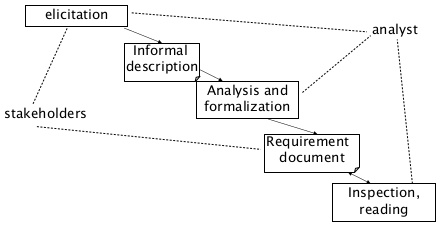
\includegraphics[scale=0.4]{images/re_phases.png}
\caption{Requirement engineering}
\end{figure}

A \textbf{requirement} is a description of a system or a service and of constraints. Requirements have different levels of abstraction and formality and they may be distinguished in functional and not functional.

Informal requirements often are not precisely stated. Ambiguous requirements may be interpreted in different ways by developers and users. In principle, requirements should be both complete and consistent.
\begin{itemize}
\item Complete: they should include descriptions of all facilities required;
\item Consistent: There should be no conflicts or contradictions in the descriptions of the system facilities.
\end{itemize}
In practice, it is impossible to produce a complete and consistent requirement document, also because there are no mathematical models or languages which can represent requirements.

\section{Defects}
\paragraph{Omission/Incompleteness}
Some information are not written. This defect is very difficult to find and fix.

\paragraph{Incorrect fact}
This defect is less difficult to find and fix. It may refer to a common knowledge.

\paragraph{Inconsistency/Ambiguity}
Some information are not strictly specified.

\paragraph{Extraneous information}
Overspecification: some information are not part of the requirement document.

\paragraph{Redundancy}
The same concept is repeated multiple times and possibly in slightly different ways which lead to ambiguity. Redundancy has to be avoided because, during the evolution of the document, it is possible to modify some concepts causing ambiguity.

\section{Techniques}
The requirement document is built using different techniques and it provides a \emph{structure}. The structure may change, order of parts is less important than precise description of parts.
\begin{enumerate}
\item Overall description;
\item Stakeholders;
\item Context diagram and interfaces;
\item Requirements
\begin{itemize}
\item Functional;
\item Non functional;
\item Domain;
\end{itemize}
\item Use case diagram;
\item Scenarios;
\item Glossary;
\item System design.
\end{enumerate}

\paragraph{Stakeholders}
A \emph{stakeholder} identifies a role or a person with an interest (stake) in the system to be built. Listing relevant stakeholders is essential to consider relevant points of view and therefore relevant requirements for the system.

\paragraph{Context diagram}
The \emph{context diagram} defines what is inside the system to be developed, what is outside and the interfaces between inside and outside. The outside entities interacting with the system are \textit{actors}. Stakeholders represent a subset of actors.

Context diagram and interfaces are essential to agree on what is the scope of the system.

\subparagraph{Interfaces}
Formal notations are an effective technique for interface specification.
Three types of interface may have to be defined:
\begin{itemize}
\item User interfaces, GUIs;
\item Procedural interfaces;
\item Data exchanged.
\end{itemize}

\paragraph{Numbering and type}
\begin{itemize}
\item Functional: General and informal description of services and behaviors provided by the system;
\item Non-functional: Constraints on how functional requirements have to be implemented.
\end{itemize}

\subparagraph{Functional}
They can be inferred after the first reading of the informal description. Functional requirements are not all at the same level (i.e.\@ complexity), in fact it is possible to introduce a hierarchy in the requirements enumeration. Naming and numbering functional requirements is very useful because it helps their management (ready, released, paid) and their testing.

\subparagraph{Non-functional}
Non-functional requirements may be more critical than functional requirements. If these are not met, the system is useless.
\begin{itemize}
\item Product requirements: requirements which specify that the delivered product must behave in a particular way (execution speed, reliability \dots);
\item Organizational requirements: requirements which are a consequence of organizational policies and procedures (process standard used, implementation requirements, \dots);
\item External requirements: requirements which arise from factors which are external to the system and its development process (interoperability requirements, legislative requirements, \dots).
\end{itemize}
Often, organizational and external requirements are taken for granted by the customer, therefore they are more difficult to extract.

ISO 9126 / ISO 25010 defines six properties of software systems associated to each function, not to the whole system.
\begin{itemize}
\item Functionality;
\item Reliability;
\item Usability \footnote{Waiting times < 0.1 sec are not perceived, while waiting > 1 are considered annoying};
\item Efficiency;
\item Maintainability;
\item Portability.
\end{itemize}

Non-functional requirements must be \emph{measurable}, otherwise they are not testable, and therefore useless.

Conflicts between different non-functional requirements are common in complex systems. It is possible to rank the requirements in order to understand which are the most important.

\subparagraph{Domain requirements}
Domain requirements are derived from the application domain and describe system characteristics and features that reflect the domain. They can be new functional requirements, constraints on existing requirements ore define specific behaviors. If domain requirements are not satisfied, the system may be unworkable.

\textbf{Understandability}: requirements are expressed in the language of the application domain and they are often not understood by software engineers developing the system.

\textbf{Implicitness}: domain specialists understand the are so well that they do not think of making the domain requirements explicit.

\paragraph{Glossary}
Glossary is important to ``standardize'' terms. A class diagram can be used to refine glossary.

\paragraph{Scenarios}
A \emph{scenario} is a sequence of steps (events) that describe a typical interaction with the system. Each step should correspond to a function. In this way, it is possible to notice if a function is missing.

A scenario is also a test case. Describing the interesting scenarios will help to perform 
coherent tests.

\paragraph{Use cases}
A \emph{use case} is a set of scenarios with common goal.

\paragraph{System design}
\emph{System design} identifies subsystems (software and not software) that compose the system.